\documentclass[]{article}

\usepackage[version = 4]{mhchem} %chem symbols and equations
\usepackage{graphicx} %graphics
\usepackage{amssymb} %math symbols
\usepackage{amsmath} %math equations
\usepackage{hyperref} %create hyperlinks: \href{link}{Word to click on}

\usepackage[sc]{mathpazo} % Use the Palatino font
\usepackage[T1]{fontenc} % Use 8-bit encoding that has 256 glyphs
\linespread{1.05} % Line spacing - Palatino needs more space between lines
\usepackage{microtype} % Slightly tweak font spacing for aesthetics
\usepackage[english]{babel} % Language hyphenation and typographical rules

\usepackage[hmarginratio=1:1,top=27mm,columnsep=20pt,left=15mm,right=15mm]{geometry} % Document margins
\usepackage[hang,small, labelfont=bf,up]{caption} % Custom captions under/above floats in tables or figures
\usepackage{enumitem} % Customized lists
\setlist[itemize]{noitemsep} % Make itemize lists more compact

\usepackage{abstract} % Allows abstract customization
\renewcommand{\abstractnamefont}{\normalfont\bfseries} % Set the "Abstract" text to bold

\usepackage{titlesec} % Allows customization of titles
\titleformat{\section}[block]{\large\centering\bfseries}{\thesection.}{1em}{} % Change the look of the section titles
\titleformat{\subsection}[block]{\bfseries}{\thesubsection.}{1em}{} % Change the look of the section titles

\usepackage{fancyhdr} % Headers and footers
\pagestyle{fancy} % All pages have headers and footers
\fancyhead{} % Blank out the default header
\fancyfoot{} % Blank out the default footer
\fancyhead[C]{Physical Chemistry $\bullet$ Oct 2019 $\bullet$ Vol. XXI, No. 1} % Custom header text
\fancyfoot[RO,LE]{\thepage} % Custom footer text

\usepackage{titling} % Customizing the title section

\renewcommand{\maketitlehookd}{%
\begin{abstract}
\noindent


%% ######

\end{abstract}
}



\begin{document}

\title{The structure of the chemical space of 1868.} 

\author{%
\textsc{Andr\'es C. Marulanda}\thanks{Corresponding author} \\[1ex]
\normalsize Universidad de Antioquia \\ % Your institution
\normalsize \href{mailto:correoAndres}{acamilo.marulanda@udea.edu.co} % Your email address
}


\maketitle


\section{Introduction}
\label{sec:intro}

During the previous months we discussed about producing an algorithm capable of making predictions about new substances based on known substances, up to some date. The initial approach was to use convolutional neural networks (CNN) to learn from some representation of the data containing also information about some periodic table (PT), similar to \cite{CNN_dH}. 

We also want to compare different PTs against Mendeleev's and against the more recent PT produced by Prof. Restrepo's group and see which one, if any, contains the most information about the substances at the time, meaning which representation can yield better predictive results for the CNN. This algorithm can then be explored in order to see what it sees and how it makes the predictions, kind of asking Mendeleev why and how he chose to predict substance properties in the way he did (for Ga and Ge, for instance).

Initially it was proposed that for this task "matrices of existence"  should be constructed, meaning that in a table a substance gets a 1 if it exists and a 0 if it doesn't, which would make the task a supervised learning one, which is the most explored type of machine learning these days.

This is, however, a somewhat loose task as the existence of a compound is in principle only limited to humanity's knowledge of it, so many possible substances in the training set would probably be wrongly labeled, which is a fundamental problem for the approach. Given this, the approach is discarded as it provides little insight into the inner structure of the chemistry of this period.

I decided then to do some exploratory data analysis (EDA) on these tables and see if some structure can directly be extracted from the data as opposed to feeding some algorithm with it right away. This has already started and the results are explored in the following sections.

The approach mentioned above still would work, however, if we used some properties of known substances as inputs (as opposed to just 1s and 0s for existence). That way we can directly ask an algorithm to predict properties of new compounds based on the (learned) structure of the chemical space and the properties of similar substances. 

In this case then, an algorithm would try to approximate the value of some property p of substance $R-X_n$.

\begin{equation}
\label{eq:eq1}
 p(R-X_n) = f( X, existent R-Y_n , PT )
\end{equation}

X being any element (characterized by its position in the given PT), Y being any element such that $\ce{R-Y_n}$ is in the dataset, and PT the periodic table considered.


\section{Data preprocessing}
\label{sec:sec2}

As initially proposed, tables were constructed in such a way that two elements X,Y appear in the same table only if there exist 2 compounds $A = R-X_n$ and $B = R-Y_n$, where if X were replaced by Y in compound A, the result would be compound B. This approximation ignores every structural factor and relies only on compositional data.

Note from this approach that n is an integer, that is, there's a problem when treating non-stoichiometric compounds. In the given dataset there are actually examples of such non-stoichiometric compounds, and so this case had to be handled properly.

This was solved in the following way: if upon duplication of all ns in the given compound this compound is stoichiometric, then work with that, otherwise discard the compound. All compunds that weren't used in this analysis due to this are stored under the out.log file, which corresponds to the output of the MPIgetTabs.py script used for the aforementioned data preprocessing. 

A total of 6145 tables was produced, and a sample of these is shown in figure \ref{fig:fig1}. The PT was the standard long-version of the PT.

\begin{figure}[h!]
  \centering
	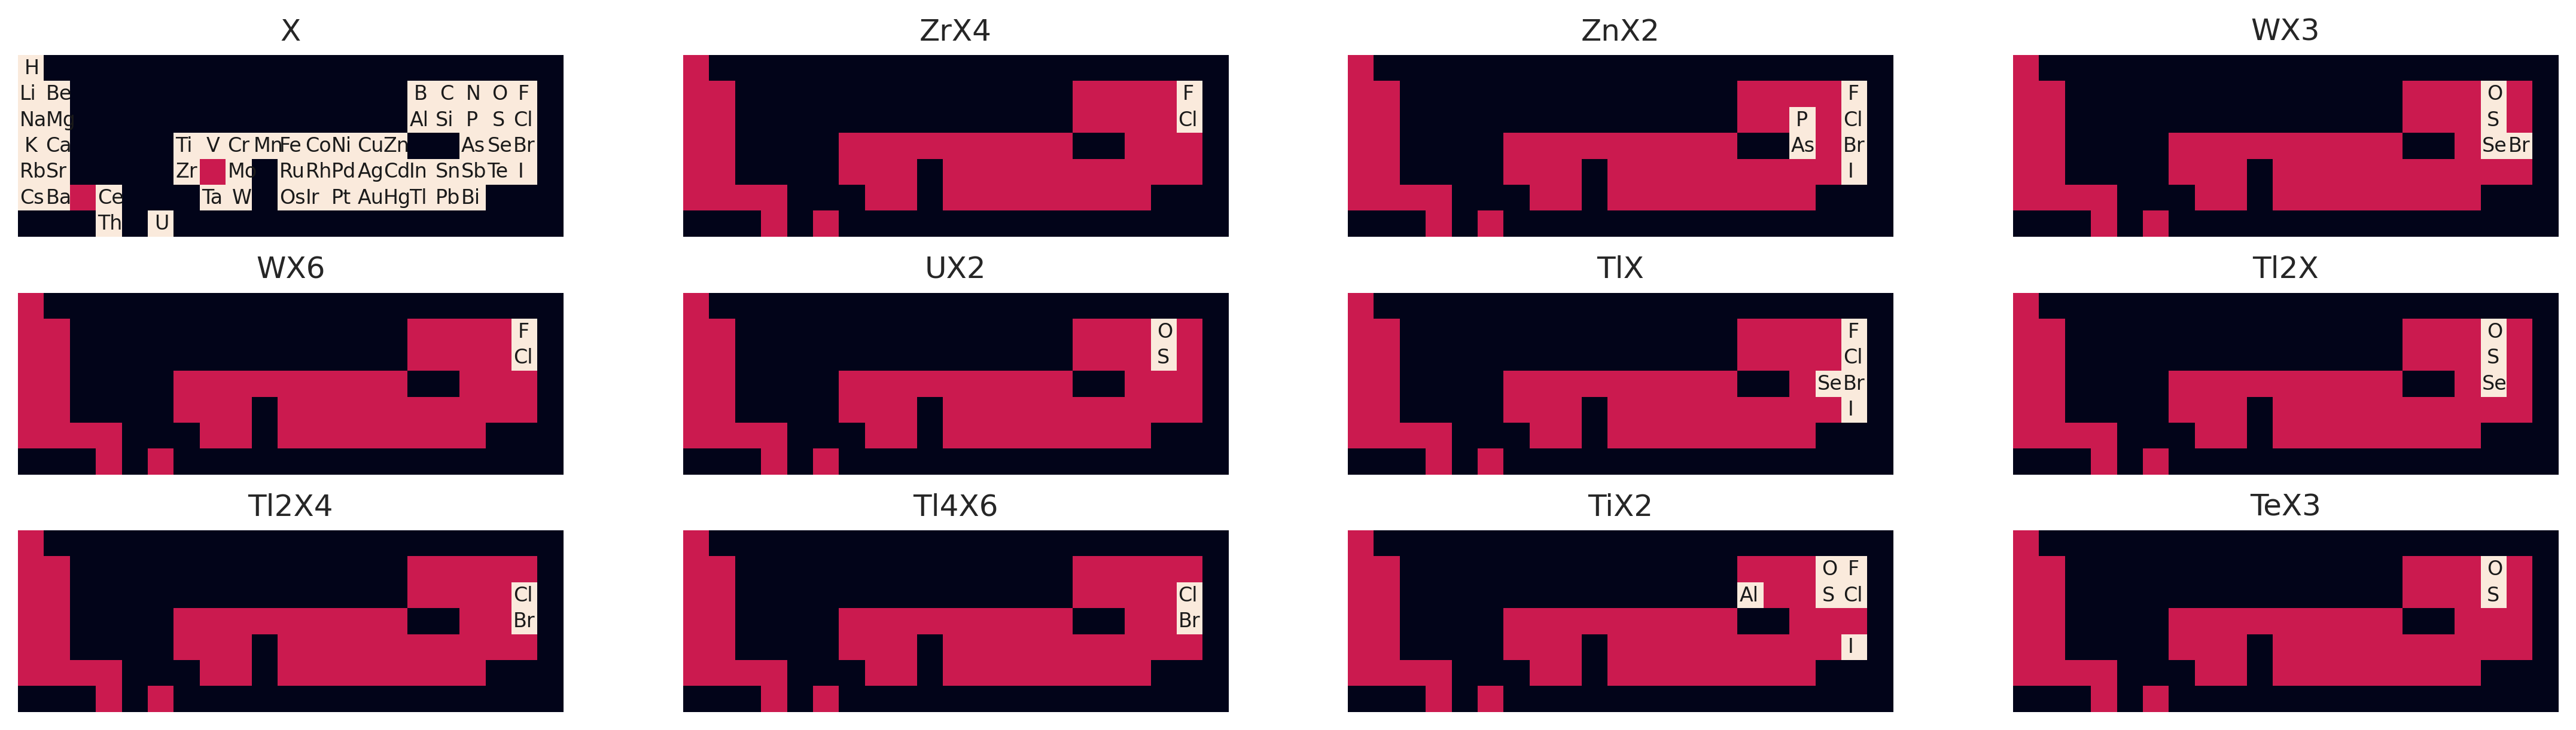
\includegraphics[width=16.0cm]{tables.png}
	\caption{Periodic table representation of the dataset.}
	\label{fig:fig1}
\end{figure}

Where purple means no element exist at this position, red means an element in this position exists in dataset, and white means there exist a compound $R-X_n$, with X being the element at this position and R the molecular fragment associated with this table. In this example, for instance, the data shows that both $\ce{ZrF4}$ and $\ce{ZrCl4}$ exist in dataset, but there exist no other compound with formula $\ce{ZrX4}$. It also shows that most lanthanides and actinides, as well as Tc, Re, Ga and Ge hadn't been discovered to this date. The vertical relationships on this side of the PT are clear from this sample.

It must be pointed out that, during preprocessing, a table is saved only if there are at least two white squares in it. Note that this implies a large loss of data as tables with only one white square correspond to unique compounds, meaning these compounds are all lost. This merits a more in-depth study and a new approach that explicitly tackles this is discussed further on.


\section{Exploratory Data Analysis (EDA)}

Having generated all the tables, we now go into data analysis. Modellation by itself must wait until I get more data (that is, substances' properties) and even then an EDA always leads to valuable insights, so that will be discussed in this section.

From figure \ref{fig:fig1} the typical vertical similarity can be spoted in the large majority of tables (vertical blocks of white squares). We may ask, however, to what extent is this vertical similarity rule followed throughout the whole dataset? That is, is it more prevalent than, for instance, horizontal or diagonal (or any other) similarity?

To answer this, the horizontal neighbor distance (HND) was calculated for each white element in each table. This is calculated as the difference in PT groups there are from one white element to another in the same table. A HND of 0 means the two elements belong in the same group, reinforcing the vertical similarity, while a larger distance implies a departure from this.

The results are then averaged throughout the tables and are shown in figure \ref{fig:fig2}.

\begin{figure}[h!]
  \centering
	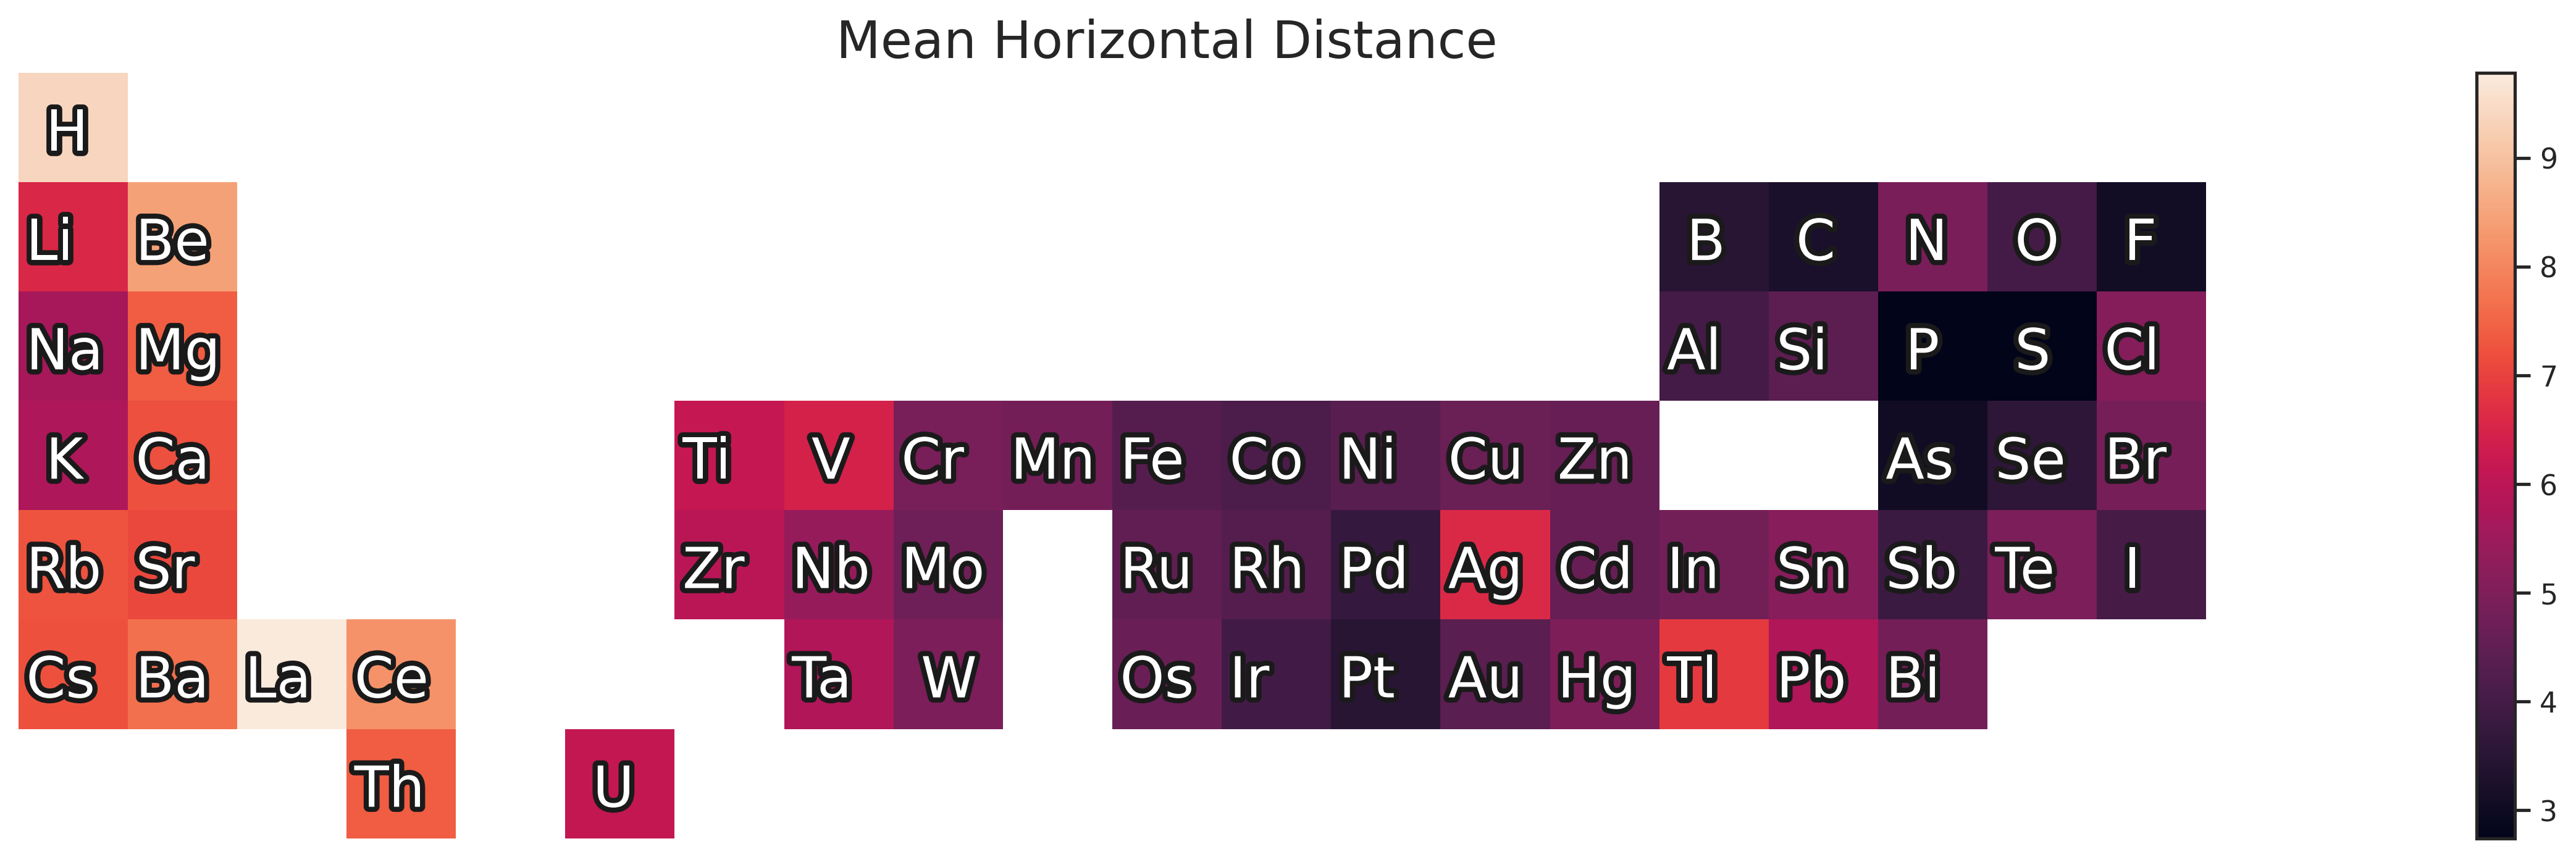
\includegraphics[width=14.0cm]{meanHND.png}
	\caption{Mean HND for the elements in the PT.}
	\label{fig:fig2}
\end{figure}

The interpretation of this plot is somewhat tricky but it clearly shows that, overall, the vertical similarities do not occur throughout the whole PT and, furthermore, this occurs more frequently to the right of the PT. Groups 1 and 2 show surprisingly high HNDs considering how chemically similar these elements are inside their group. This is explained considering the metallic character of these elements, which is in some aspects similar to that of transition metals.

We can calculate a number of other different distances, but I think this is the most important as the PT is constructed on the basis of order and similarity, with the similarity expresed as a strictly vertical one on this representation. We may now construct a new PT by optimization of this quantity, which would lead to a PT where HND is minimized while preserving atomic number ordering. This should naturally lead to a more complete PT, and would allow a comparison between systems.

This might be done using genetic algorithms, which are perfect for these kind of problems where an exhaustive exploration of the space of configurations is impossible and the mixing of configurations is somewhat straightforward.

\begin{figure}[h!]
  \centering
	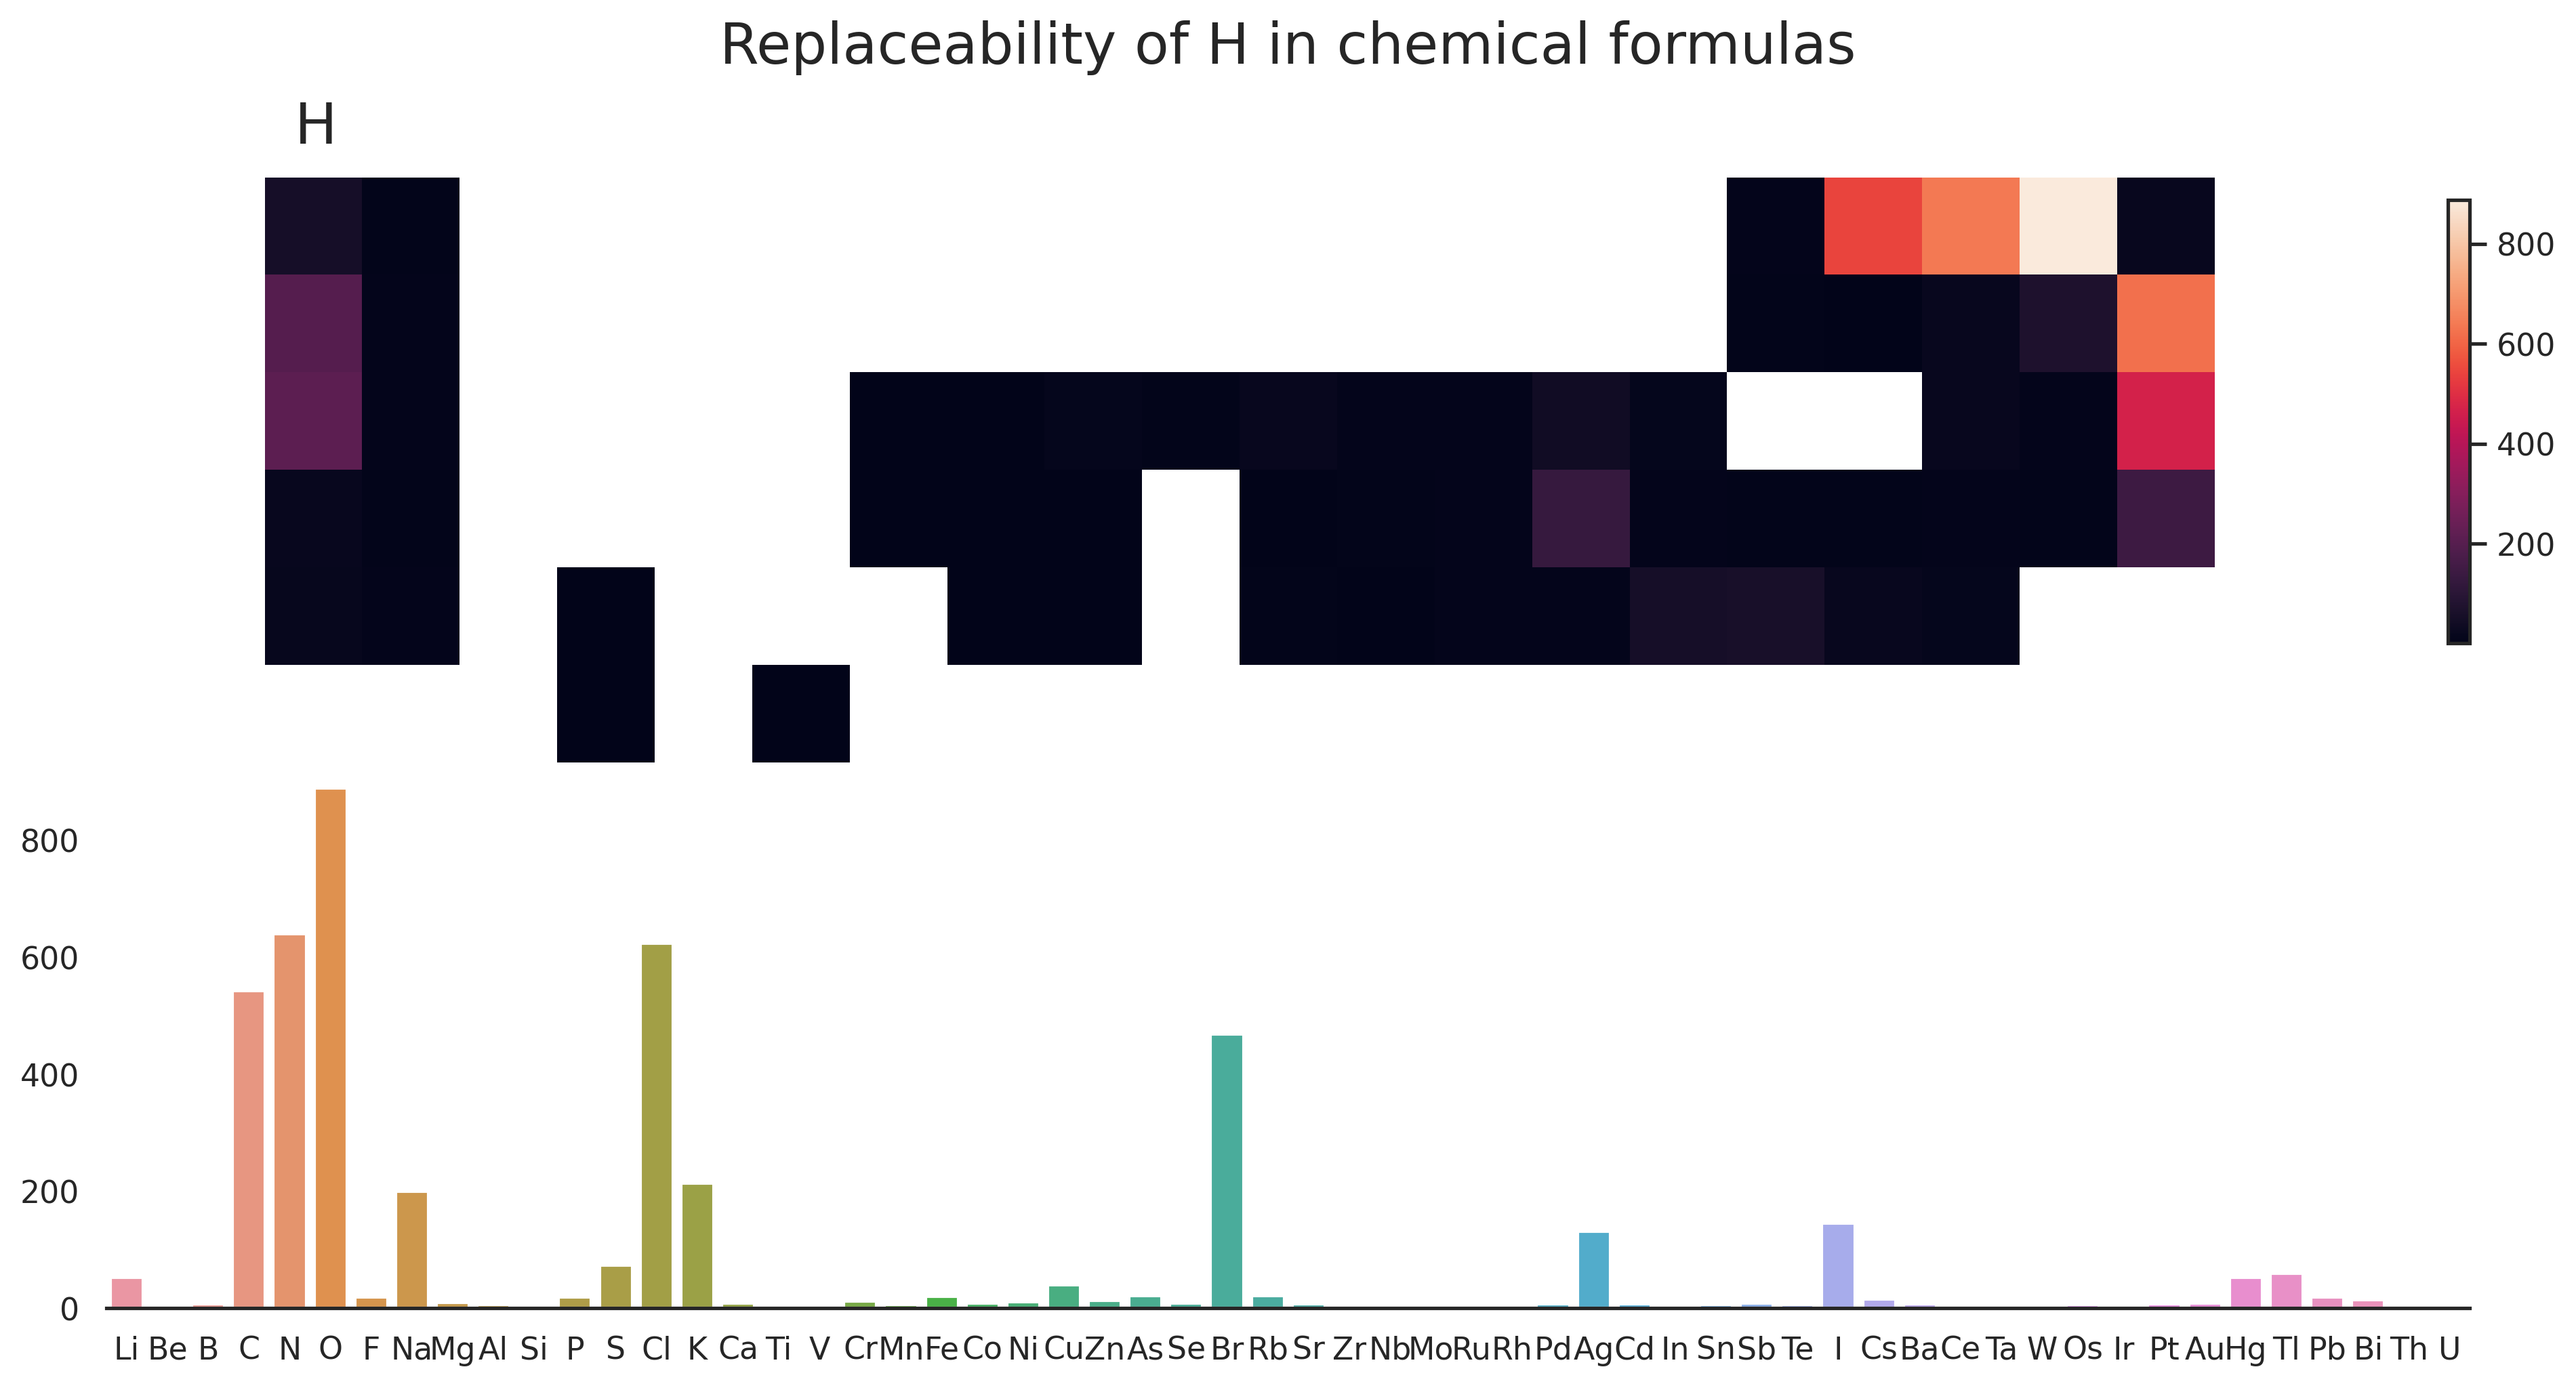
\includegraphics[width=13.0cm]{replace_H.png}
	\caption{Replaceability of H in dataset. Both plots show the same data in different formats. a) PT format showing vertical relationships and b) Barplot showing elements in atomic number order, bar height is number of times H and this element appear in the same table.}
	\label{fig:fig3}
\end{figure}

A more individual exploration can be done using the same data. Particularly, the degree of replaceability was calculated for each pair of elements as the number of times both elements appear in the same table. From this, we can obtain some more detailed insights about the relationships between elements, as shown in figure \ref{fig:fig3}.

It can clearly be seen that H is, under our approximation, more similar to C, N and O, and the halogens (except F). A similarity with the halogens are expected, as in most of organic chemistry these appear as substituents of H, but the similarity to C, N and O must be further explored.

As a quick comment, some of the substances responsible of the high H-O replaceability are: 
$\ce{SX2}$, $\ce{OTlX}$, $\ce{NX3}$, $\ce{MoOX}$, $\ce{MnOX}$. These show that this result is actually due to the presence of metallic oxides, hydroxides and hydrides, and happens with elements with many oxidation states, such as transition metals and other non-metals such as S and N.

To show the power of these plots, another example is brought into play (figure \ref{fig:fig4}).

\begin{figure}[h!]
  \centering
	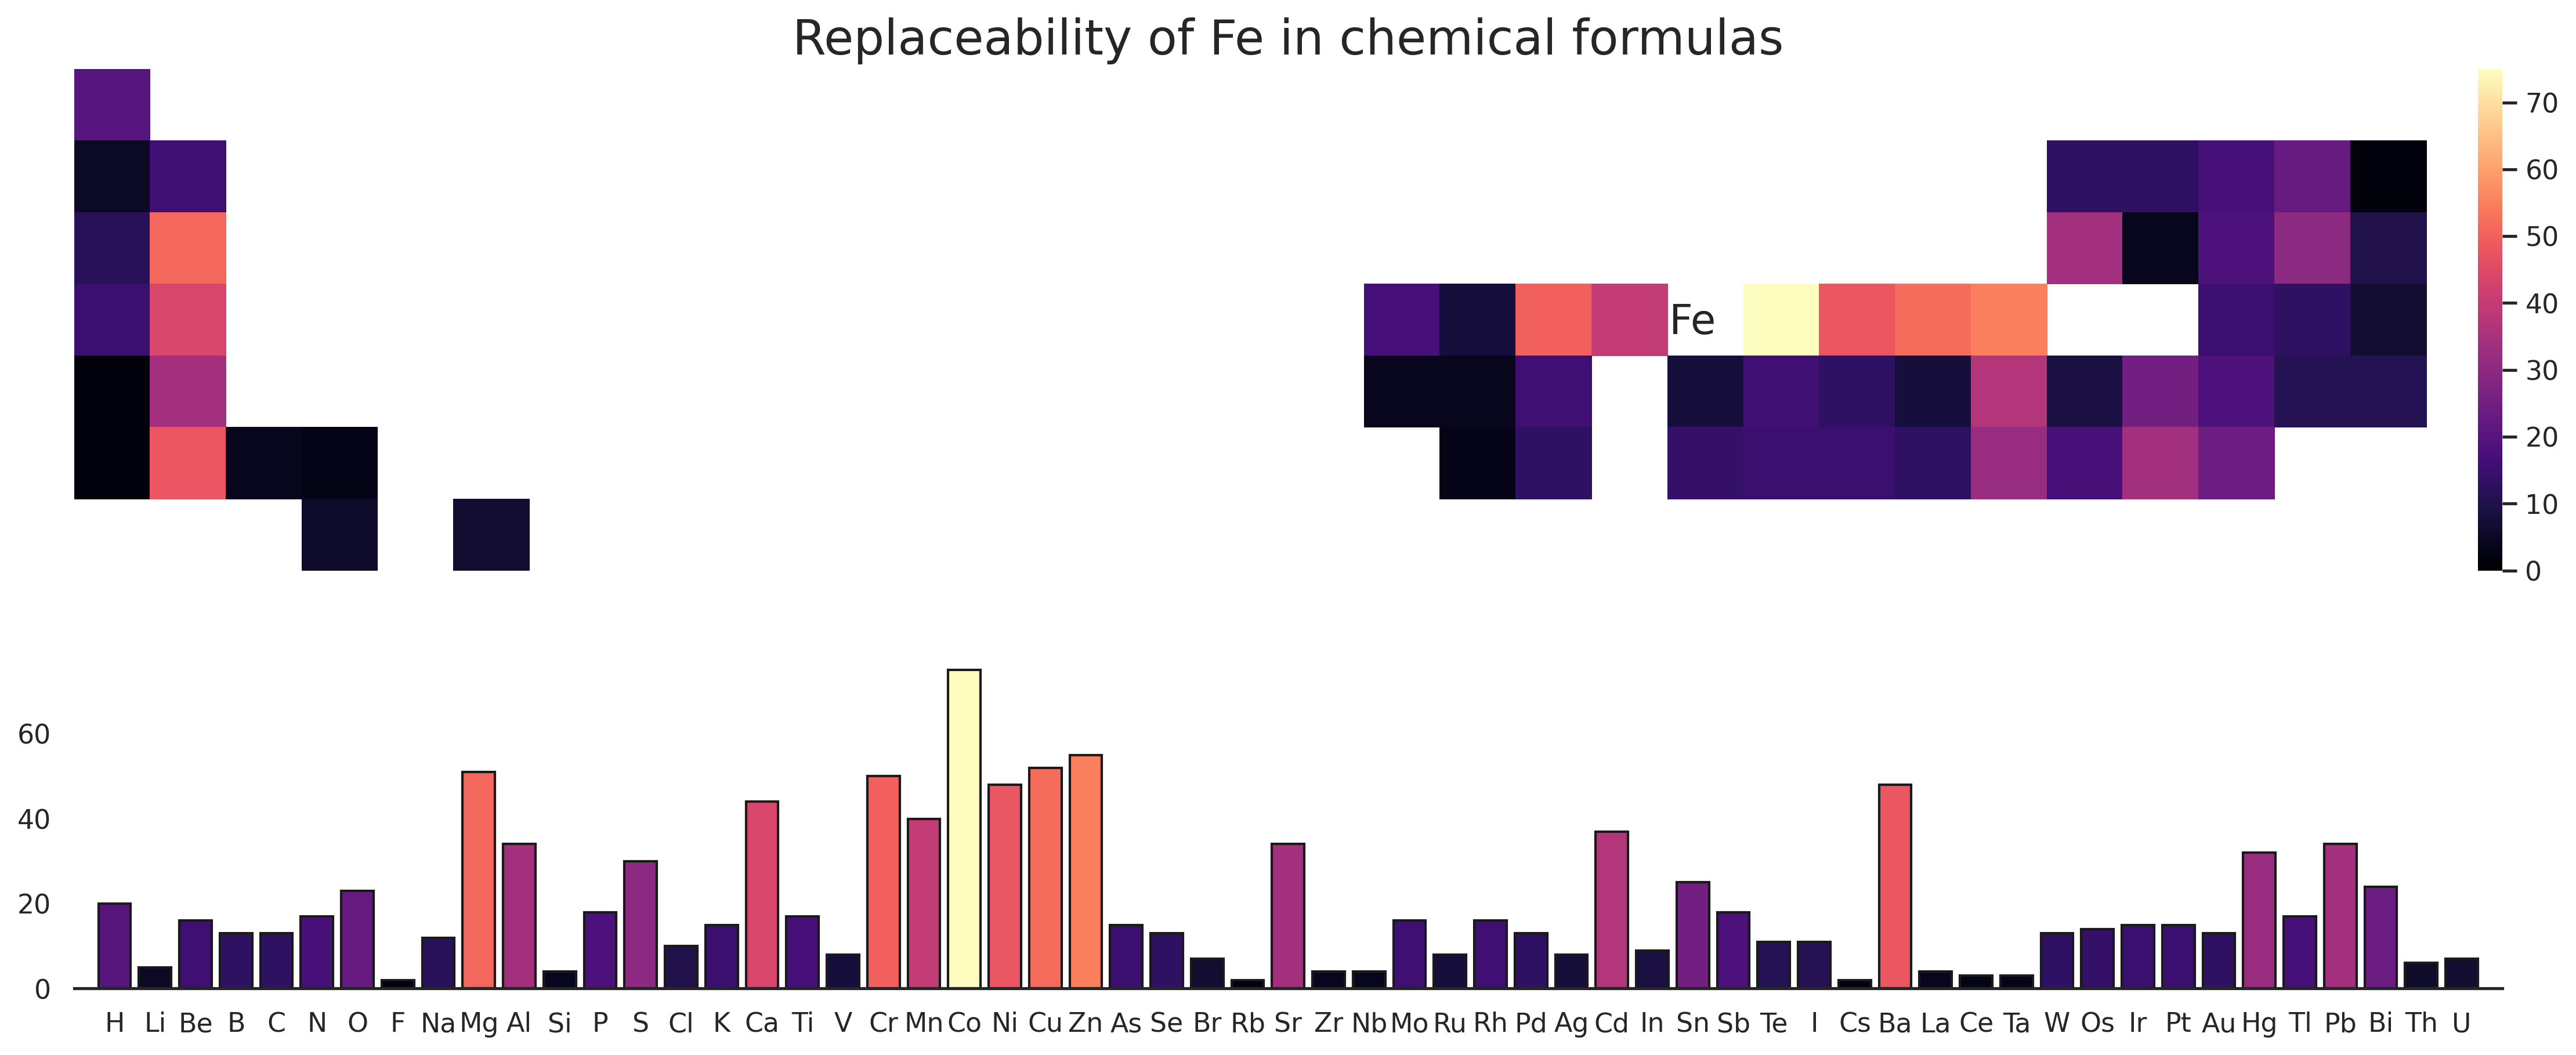
\includegraphics[width=13.0cm]{replace_Fe.png}
	\caption{Replaceability of Fe in dataset.}
	\label{fig:fig4}
\end{figure}

The replaceability plot for Fe shows that, for this element, the similarity is mostly horizontal along the 4th period transition metals, but it also shows a large similarity with alkaline earth elements. This result is, I think, non trivial and deserves a more in-depth exploration. Some questions arise as, for instance, can a new PT be constructed, in such a way that this information is mre explicitly given? If not, is there some particular reason (probably a topological one) for this?.

As an additional observation, the plots for alkaline elements (Na for instance) do not show such a marked similarity to transition metals and are instead more cluttered around group 1 of PT.

We could go on and do one of these plots for each element, but this becomes quite tedious as we would have to analize more than 90 of these individually. Instead we can unravel the periodic table representations into a 1-dimensional format, do some normalization on this replaceability measure, and procede to concatenate all 1-D arrays into one large square matrix, as shown in figure \ref{fig:fig5}. This ultimately looks much like a correlation matrix as it states element-wise relationships between pairs of elements in a more concise format.

The details of the normalization are important as it determines what is shown on the figure. In this case each row of the matrix was divided by the maximum value of said row. This value naturally corresponds to the same element as the row, which justifies the observation that the diagonal of the matrix is all ones.

Due to the normalization used, the matrix is not symmetric, which means the matrix doesn't equal its transpose. As an example, take the couple La-Fe. As can be seen, the row corresponding to La has a high value (near 1) at the Fe column, meaning La can be replaced by Fe most of the time (within this dataset). When we look at the Fe row, the value corresponding to 1 is one of the lowest, meaning Fe can not be replaced by La most of the time. 

The unidirectionality of these relationships is important as it may lead to several conclusions (drawn naively only from this study), namely:

\begin{itemize}
	\item The chemistry of La wasn't as explored as that of Fe at the time. This can be thought of in sociological terms, as an exploration of the new element (La) limited to trying to copy the chemistry of a seemingly similar element (Fe).
	\item Or possibly the chemistry of La is more restricted than that of Fe, meaning possibly that the oxidation numbers for La are only a subset of those for Fe.
\end{itemize}

\begin{figure}[h!]
  \centering
	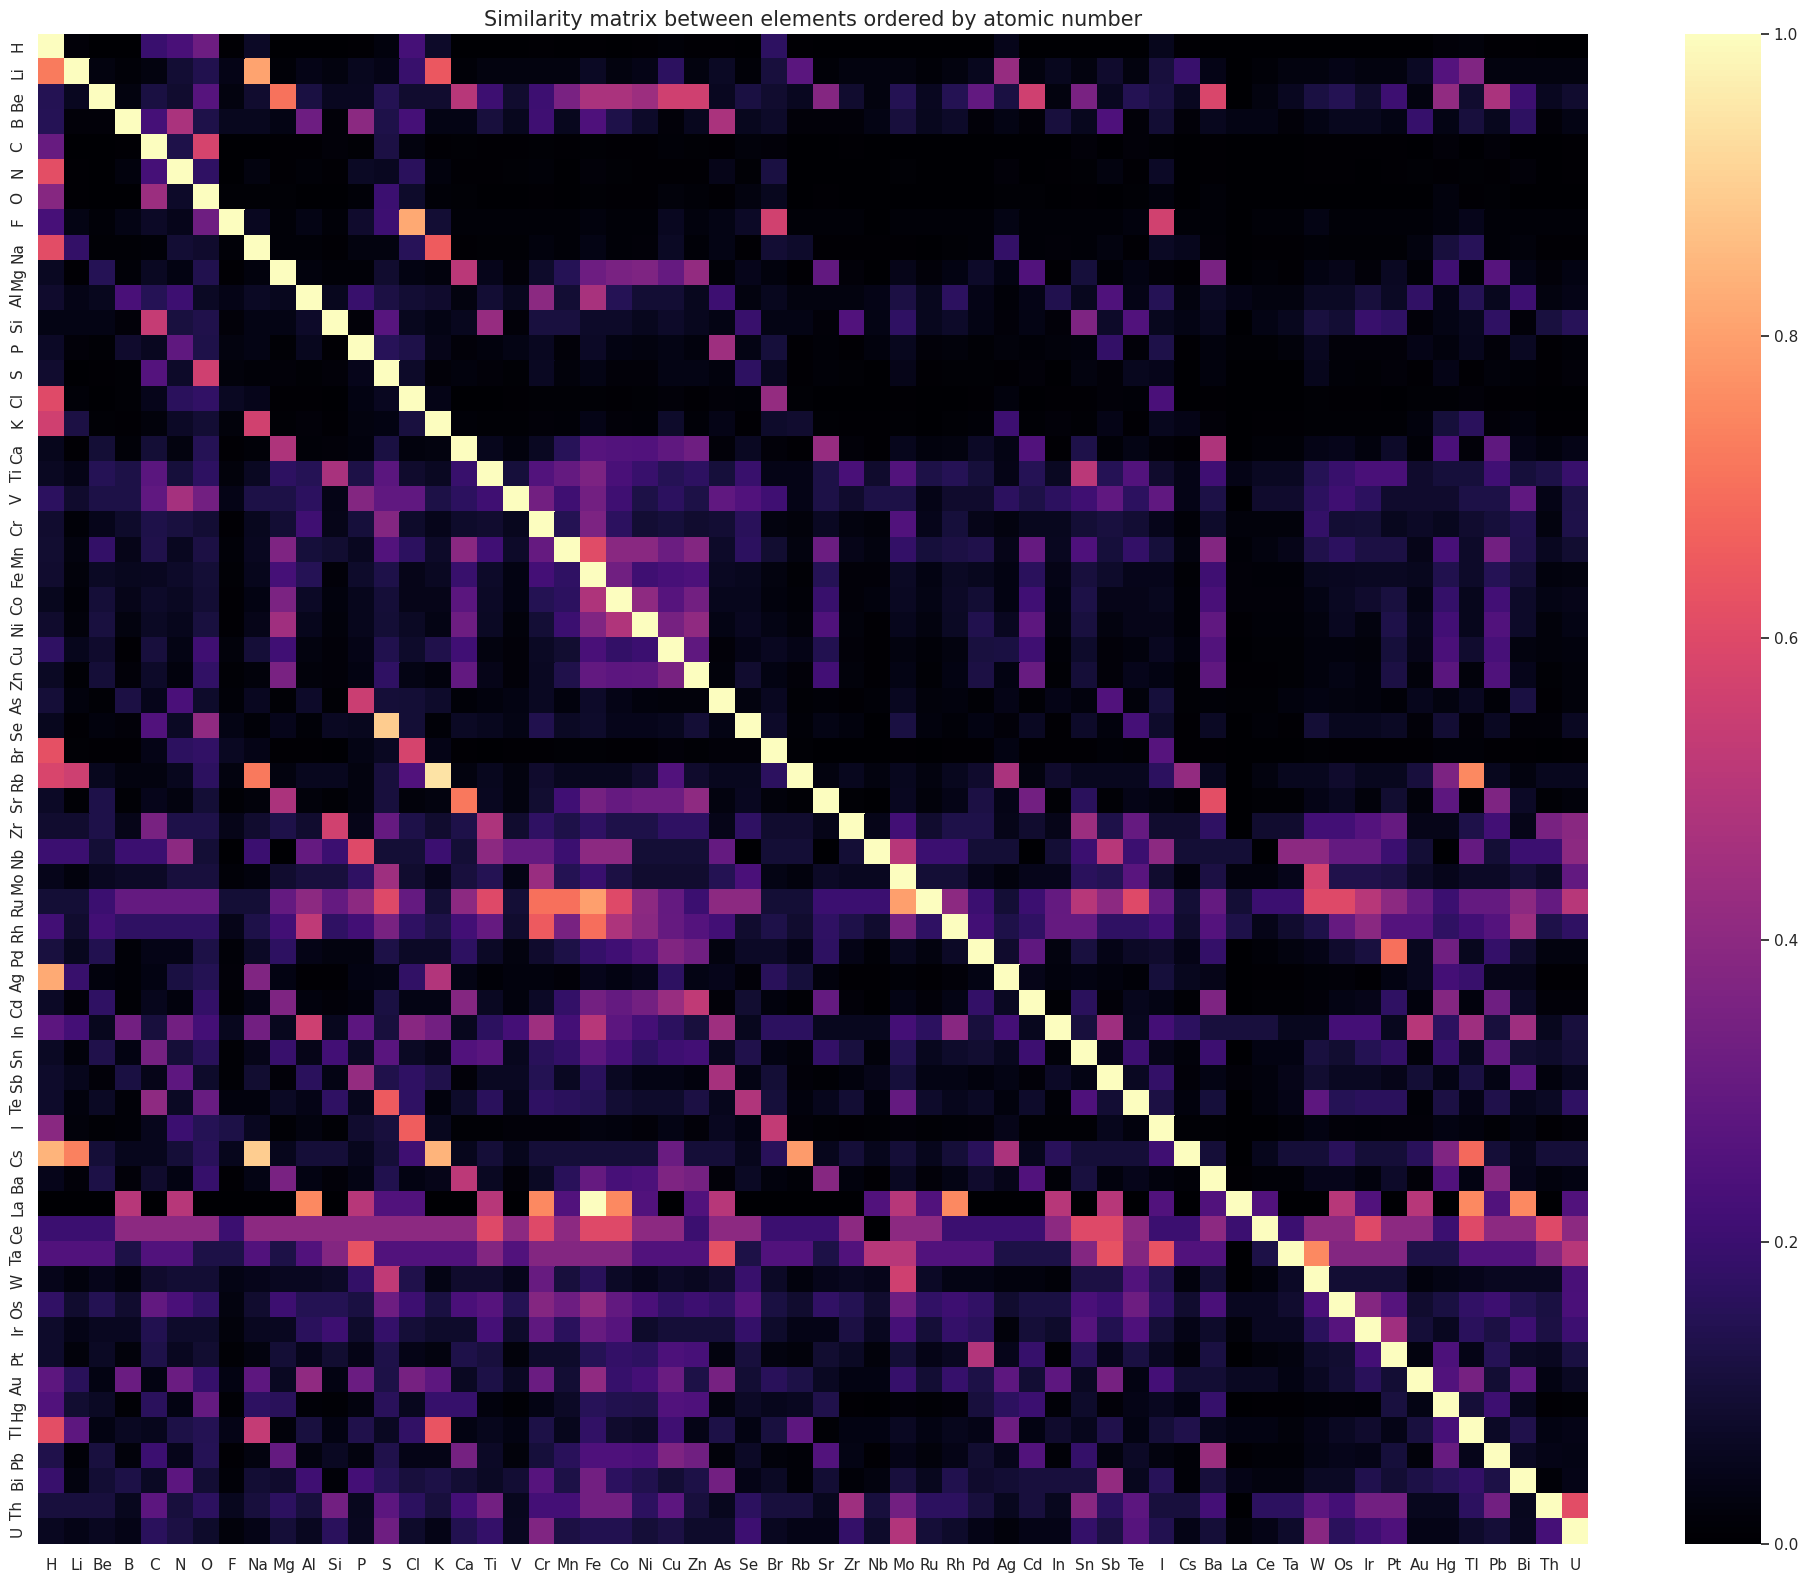
\includegraphics[width=18.0cm]{matrix.png}
	\caption{Replaceability of Fe in dataset.}
	\label{fig:fig5}
\end{figure}

In more general terms, some substructures can be seen within the matrix such as, for instance, vertical, horizontal and diagonal lines, which explicitly suggest the higher structure the PT is intended to capture. Again, some optimization work can be performed on this matrix, similar to \cite{Glawe_2016}. The present paper could in fact be an extension of this, as it takes a very similar concept and extends it from inorganic solids to all known substances (up to some date).

Aside from such loose statements, it has to be pointed out that this matrix gives important information about the dataset, which ultimately speaks about the chemistry of the moment. This must be more thoroughly analized, but I think it already is an important product of this project.

\section{Further work}

As already pointed out, the data preprocessing presented here represents a huge loss of data as it doesn't exploit the full structure of the chemical compositional formulas and disregards a number of formulas as these are unique in the sense that no replacement of any atom in the formula leads to another compound in the dataset. It must be noted, however, that this preprocesing was initially conceived for a tabular representation intended to feed a CNN. A different preprocessing would require a different algorithm.

A new approach, one which takes into account these failures and aims to exploit the full structure of the dataset, relies on a similar idea as automatic computer text generation using recurrent neural networks (RNN). Under this approach, an RNN is exposed to a corpus of raw text and asked to predict what the next word will be, based on some current state. For instance, a state may be "Colombian people speak" and the algorithm would be expected to say "spanish" with high probability. More on this on \href{https://karpathy.github.io/2015/05/21/rnn-effectiveness/}{Karpathy} \cite{text_gen_rnn}.

The power of this approach relies on the fact that the algorithm needs to learn to structure text in the given language, remember previous information, and be aware of context. A direct bridge to chemistry is constructed when we think of compositional formulas as a new language, where based on the context (e.g. some information about the formula) we'd like our model to predict what elements and in what quantities could complete them. An example of this is having "$\ce{H2}$" as an input. The output would be $\ce{H2O}$, or $\ce{H2S}$ with high probability, but other results such as $\ce{H2Br}$ shouldn't be as likely.

It is in this sense that RNNs could help exploit the full structure of the dataset without the need of any additional data. Naturally, the interesting part comes after the algorithm has been trained. At this stage we have to analyze the strcuture of this network, the results it produces, among other tests.



\renewcommand\refname{Referencias}
\bibliography{bib}
\bibliographystyle{ieeetr}

\end{document}             % End of document.

